%!TEX root = ../prueba.tex
En este capítulo se describe de forma general la base de datos y las decisiones que se tomaron en su diseño y que no están consideradas en la etapa de análisis, como por ejemplo, el uso de algunas banderas o atributos que permitan verificar, de forma eficiente, el estado o las acciones a realizar cuando se presenta una pantalla en la aplicación móvil o en la aplicación web.

\section{Notación}
En está sección se describen los tipos de tablas que se pueden encontrar en el diagrama de la figura \ref{fig:bd} y la notación utilizada para crear los nombres de las tablas y de sus columnas.

\subsection{Asignación de nombres y atributos}
\begin{description}
	\item[Tablas] Las tablas son nombradas a partir del siguiente esquema : \textit{txxyy\_zz} donde \textit{xx} indica el módulo al que pertenece la tabla los cuales pueden ser:
		\begin{Citemize}
			\item \textit{mau} Módulo de Autenticación.
			\item \textit{mps} Módulo del Proveedor del Servicio.
			\item \textit{mor} Módulo de Órdenes.
			\item \textit{mpg} Módulo de Pagos.
		\end{Citemize}
		\textit{yy} es un dígito que puede ser desde el número \textit{00} al \textit{99}.
		\textit{zz} es un nombre para identificar a la tabla generalmente haciendo referencia a un término de negocio.
	\item[Columnas:] \hspace{1pt}
		\begin{Citemize}
			\item \textit{id\_xx} Se utiliza para identificar la llave primaria de una tabla y \textit{xx} es el nombre de la tabla o el nombre de la llave foránea a la que hace referencia.
			\item \textit{nb\_xx} Se utiliza para identificar una columna que indica el nombre o el sustantivo propio con el que es posible conocer un registro de la tabla.
			\item \textit{tx\_xx} Se utiliza para indicar que la columna es texto.
			\item \textit{st\_xx} Se utiliza para indicar que la columna es de tipo booleano o entero y generalmente indica un estado de un registro de la tabla.
			\item \textit{fh\_xx} Se utiliza para indicar que la columna representa una fecha.
		\end{Citemize}

\end{description}


\subsection{Tipos de Tablas}
	\begin{Citemize}
		\item 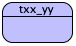
\includegraphics[height=20pt]{template/img/table} Es una tabla de color azul que representa una entidad fuerte o de negocio como en este caso puede ser \getElementById[Entidad]{local} o \getElementById[Entidad]{producto}. Si este tipo de tabla sólo tiene una llave(representada en el diagrama con negritas y un signo $+$) entonces se hará uso de una secuencia para mantener controlado el identificador que le puede ser asignado a los registros de este tipo de tablas.
		\item 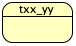
\includegraphics[height=20pt]{template/img/catalogo} Es una tabla de color amarillo que representa un catálogo en el sistema que se puede asociar a una entidad fuerta o de negocio como en este caso puede ser \getElementById[Entidad]{tipoOrden} o \getElementById[Entidad]{tipoProducto}. Este tipo de tablas no hacen uso de una secuencia dado que sus registros son insertados de forma controlada al crear la base de datos.
		\item 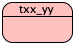
\includegraphics[height=20pt]{template/img/stateMachine} Es una tabla de color rosa en la que se almacenan los estados que intervienen o indican la condición de los registros de una entidad fuerte o de negocio. Este tipo de tablas no hacen uso de una secuencia dado que sus registros son insertados de forma controlada al crear la base de datos.
	\end{Citemize}


\section{Diagrama Relacional}
En esta sección se presenta el diagrama entidad relación de la base de datos\footnote{ver figura \ref{fig:bd}}.

\begin{figure}[hbtp!]
	\begin{center}
		\fbox{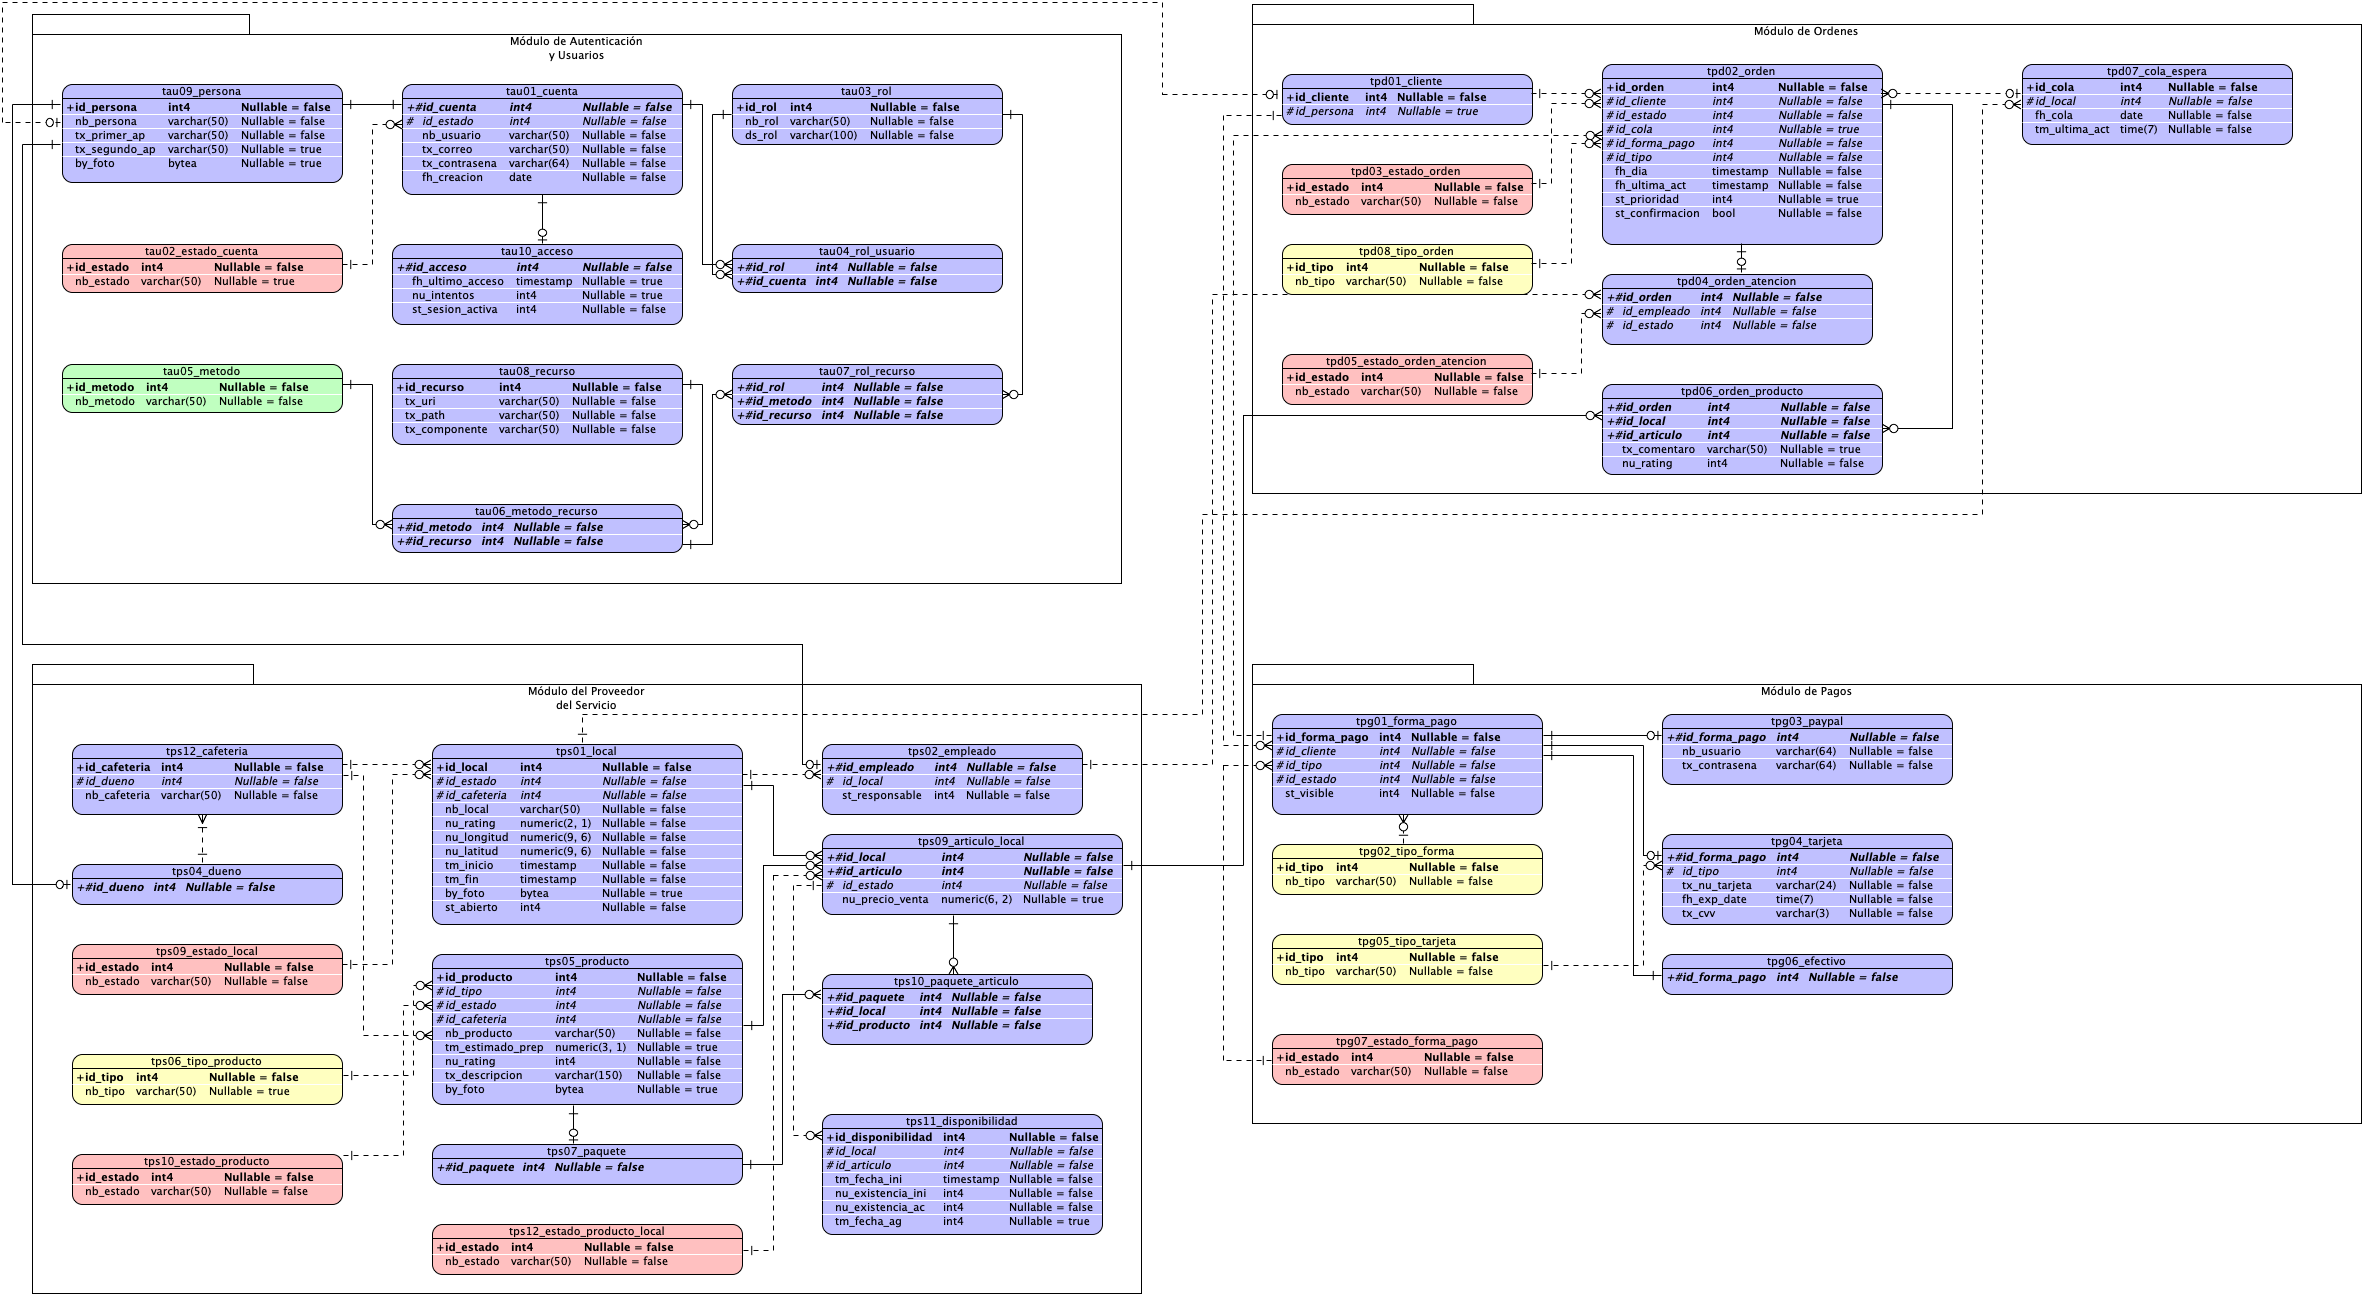
\includegraphics[angle=90,width=\textwidth,height=\textheight]{img/BD}}
		\caption{Diagrama ER de la Base de Datos}
		\label{fig:bd}
	\end{center}
\end{figure}
